\section*{Цель работы}

Целью работы  является моделирование системы, состоящей из генератора, буфера и
обслуживающего аппарата. Генератор выдает сообщения, распределенные по
равномерному закону, они приходят в память, обслуживающий аппарат обрабатывает
каждое из них согласно нормальному распределению. Необходимо определить
оптимальную длину очереди, при которой не будет потерянных сообщений.
Использовать принципы $\Delta t$ и событийный. Задаваемая часть сообщений
попадает в очередь повторно.

\section*{Принципы организации управляющей программы}
\vspace{-1\baselineskip}
\subsection*{Принцип $\Delta t$}

Данный принцип заключается в последовательном анализе состояний всех блоков в
момент $t + \Delta t$ по заданному состоянию блоков в момент $t$. При этом
новое состояние блоков определяется в соответствии с их алгоритмическим
описанием с учетом действующих случайных факторов, задаваемых распределениями
вероятности. В результате такого анализа принимается решение о том, какие
общесистемные события должны имитироваться программной моделью на данный момент
времени.

Основной недостаток этого принципа: значительные затраты машинного времени на
реализацию моделирования системы. А при недостаточно малом $\Delta t$
появляется опасность пропуска отдельных событий в системе, что исключает
возможность получения адекватных результатов при моделировании.

\subsection*{Событийный принцип}

Характерное свойство систем обработки информации заключается в том, что
состояния отдельных устройств изменяются в дискретные моменты времени,
совпадающие с моментами времени поступления сообщений в систему, времени
поступления окончания задачи, времени поступления аварийных сигналов и т.д.
Поэтому моделирование и продвижение времени в системе удобно проводить,
используя событийный принцип, при котором состояние всех блоков имитационной
модели анализируется лишь в момент появления какого-либо события. Момент
поступления следующего события определяется минимальным значением из списка
будущих событий, представляющего собой совокупность моментов ближайшего
изменения состояния каждого из блоков системы.

\section*{Моделируемая система}

\begin{figure}[h]
    \centering
    \def\svgwidth{\textwidth}
    \input{scheme.pdf_tex}
    \caption{Схема моделируемой системы}
\end{figure}

\clearpage

\section*{Текст программы}
\begin{lstlisting}[caption={Реализация элементов системы}, language=c++]
class Model
{
    public:
        Model(std::string name);
        virtual ~Model(void) = 0;

        virtual const std::string &getName(void) const;

        virtual void
        setModifier(std::shared_ptr<RequestModifier>);
        virtual std::shared_ptr<RequestModifier>
        getModifier(void) const;

    private:
        const std::string name;
        std::shared_ptr<RequestModifier> modifier;
};

class Request
{
    public:
        virtual ~Request(void) = 0;
};

class Sender;

class Receiver
{
    public:
        Receiver(std::shared_ptr<Pipe> pipe);
        virtual ~Receiver(void) = 0;

        void connectInPipe(std::shared_ptr<Pipe> pipe);
        std::shared_ptr<Pipe> inpipe(void);
        void askSender(void);

        void registerSender(std::shared_ptr<Sender> sender);

    private:
        std::shared_ptr<Pipe> _inpipe;
        std::list<std::shared_ptr<Sender>> _senders;
};

class Sender
{
    public:
        Sender(std::shared_ptr<Pipe> pipe);
        virtual ~Sender(void) = 0;

        void connectOutPipe(std::shared_ptr<Pipe> pipe);
        std::shared_ptr<Pipe> outpipe(void);

        virtual void callback(void) = 0;

    private:
        std::shared_ptr<Pipe> _outpipe;
};

class Runner
{
    public:
        virtual ~Runner(void) = default;
        virtual void run(void) = 0;
};

class BasicPipe : public Pipe
{
    public:
        BasicPipe(std::string name);
        virtual ~BasicPipe(void) override = default;

        virtual bool empty(void) const override;
        virtual bool push(std::shared_ptr<Request>) override;
        virtual std::shared_ptr<Request> pop(void) override;

        virtual void newSet(void) override;
        virtual void dropCurrentSet(void) override;
        virtual void clear(void) override;

    private:
        std::mutex mutex;
        std::list<std::list<std::shared_ptr<Request>>> sets;
};

class Buffer : public Model, public Sender, public Receiver
{
    public:
        Buffer(std::string name, const size_t size,
               std::shared_ptr<Pipe> inpipe,
               std::shared_ptr<Pipe> outpipe);
        virtual ~Buffer(void) override = default;

        virtual size_t read(void);
        virtual size_t send(size_t amount = 1);

        virtual size_t used(void) const;

        virtual void callback(void) override;

    private:
        const size_t size;
        std::list<std::shared_ptr<Request>> memory;
        std::mutex mutex;
};

class Gate : public Model, public Receiver
{
    public:
        class Out : public Model, public Sender
        {
            public:
                Out(std::string name,
                    std::shared_ptr<Pipe> outpipe);
                virtual ~Out(void) override = default;

                virtual bool send(std::shared_ptr<Request>);

                virtual void callback(void) override;
        };

    public:
        Gate(std::string name, std::shared_ptr<Pipe> inpipe,
             std::list<std::shared_ptr<Pipe>> outpipes);
        virtual ~Gate(void) override = default;

        virtual void
        setModifier(std::shared_ptr<RequestModifier>)
        override;

        virtual bool read(void);
        virtual bool redirect(std::string name);
        virtual const std::list<std::string> &list(void);

    private:
        std::list<std::shared_ptr<Out>> outs;
        std::list<std::string> names;
        std::shared_ptr<Request> current = nullptr;
};

class RequestCreator
{
    public:
        virtual ~RequestCreator(void) = default;
        virtual std::shared_ptr<Request> create(void) = 0;
};

class Generator : public Model, public Sender
{
    public:
        Generator(std::string name,
                  std::shared_ptr<Pipe> outpipe = nullptr);
        virtual ~Generator(void) override = default;
        virtual void callback(void) override;

        virtual void
        setCreator(std::shared_ptr<RequestCreator> creator);

        virtual void generate(const size_t amount = 1);

    private:
        std::shared_ptr<RequestCreator> cretator = nullptr;
};

class Processor : public Model, public Sender,
                  public Receiver
{
    public:
        Processor(std::string name,
                  std::shared_ptr<Pipe> inpipe = nullptr,
                  std::shared_ptr<Pipe> outpipe = nullptr);
        virtual ~Processor(void) override = default;

        virtual bool read(void);
        virtual bool isActive(void) const;
        virtual bool release(void);

        virtual void callback(void) override;

    private:
        std::shared_ptr<Request> active = nullptr;
        std::list<std::shared_ptr<Request>> current;
};

class Terminator : public Model, public Receiver
{
    public:
        Terminator(std::string name,
                   std::shared_ptr<Pipe> inpipe = nullptr);
        virtual ~Terminator(void) override = default;

        virtual void read(void);
        std::list<std::shared_ptr<Request>> getDone(void);

    private:
        std::list<std::shared_ptr<Request>> done;
};

class StatatisticsBlock : public Model
{
    public:
        using ModelMap = 
        std::unordered_map<std::string,
                           std::shared_ptr<Model>>;
        class Strategy
        {
            public:
                virtual ~Strategy(void) = default;
                virtual void
                execute(const ModelMap &model) = 0;
        };

    public:
        StatatisticsBlock(std::string name,
                          std::list<std::shared_ptr<Model>>);
        virtual ~StatatisticsBlock(void) override = default;

        virtual void
        registerStrategy(std::shared_ptr<Strategy> strategy);
        virtual void write(void);

    private:
        std::list<std::shared_ptr<Strategy>> strategies;
        ModelMap map;
};
\end{lstlisting}

\begin{lstlisting}[caption={Реализация подхода $\Delta t$}, language=c++]
class TimeModel
{
    public:
        virtual ~TimeModel(void) = default;
        virtual size_t priority(void) = 0;
        virtual void tick(double time) = 0;
        virtual void
        setModifier(std::shared_ptr<RequestModifier>) = 0;
};

class TimeRunner : public Runner
{
    public:
        TimeRunner(size_t requests, double time, double step,
                   std::shared_ptr<TimeRequestModifier>,
                   std::list<std::shared_ptr<TimeModel>>);
        virtual ~TimeRunner(void) override = default;

        virtual void run(void) override;

    private:
        const size_t requests;
        const double end;
        const double step;
        std::shared_ptr<TimeRequestModifier> modifier;
        std::map<size_t,
                 std::list<std::shared_ptr<TimeModel>>> \
        items;
};

TimeRunner::TimeRunner(size_t requests, double time,
                       double step,
                       std::shared_ptr<TimeRequestModifier>,
                       std::list<std::shared_ptr<TimeModel>>)
    : requests(requests), end(std::abs(time)),
      step(std::abs(step)), modifier(modifier)
{
    if (nullptr == this->modifier)
        throw std::logic_error("Nullptr modifier");

    for (auto &item : items)
    {
        if (nullptr == item)
            throw std::logic_error("Nullptr modifier");

        auto iter = this->items.find(item->priority());

        if (this->items.end() == iter)
            this->items.emplace(item->priority(),
            std::list<std::shared_ptr<TimeModel>>({item}));
        else
            (*iter).second.push_back(item);
    }
}

void TimeRunner::run(void)
{
    double time = 0;
    this->modifier->setTime(time);
    auto modifier = this->modifier->getModifier();

    for (auto &pair : this->items)
        for (auto &item : pair.second)
            item->setModifier(modifier);

    for (; this->end > time
           && this->requests > this->modifier->getPassed();
           time += this->step)
        for (auto &pair : this->items)
            for (auto &item : pair.second)
                item->tick(time);
}
\end{lstlisting}

\begin{lstlisting}[caption={Реализация событийного подхода}, language=c++]
class EventModel
{
    public:
        virtual ~EventModel(void) = default;
        virtual void event(void) = 0;
        virtual double nextEvent(void) const = 0;
        virtual void generateNextEvent(void) = 0;
        virtual void
        setModifier(std::shared_ptr<RequestModifier>) = 0;
};

class EventRunner : public Runner
{
    public:
        EventRunner(size_t requests, double time,
                    std::shared_ptr<EventRequestModifier>,
                    std::list<std::shared_ptr<EventModel>>);
        virtual ~EventRunner(void) override = default;

        virtual void run(void) override;

    private:
        const size_t requests;
        const double end;
        std::shared_ptr<EventRequestModifier> modifier;
        std::list<std::shared_ptr<EventModel>> items;
};

EventRunner::EventRunner(size_t requests, double time,
                         std::shared_ptr<EventRequestModifier>,
                         std::list<std::shared_ptr<EventModel>>)
    : requests(requests), end(time), modifier(modifier),
      items(items)
{
    if (nullptr == this->modifier)
        throw std::logic_error("Nullptr modifier");

    for (auto &item : items)
        if (nullptr == item)
            throw std::logic_error("Nullptr modifier");
}

void EventRunner::run(void)
{
    double time = 0;
    this->modifier->setTime(time);
    auto modifier = this->modifier->getModifier();

    for (auto &item : this->items)
        item->setModifier(modifier);

    while (this->end > time
           && this->requests > this->modifier->getPassed())
    {
        auto iter = this->items.begin(), next = iter;

        for (; this->items.end() != iter; ++iter)
            if ((*iter)->nextEvent() < (*next)->nextEvent())
                next = iter;

        auto model = *next;
        time = model->nextEvent();
        model->event();
        model->generateNextEvent();
    }
}
\end{lstlisting}


\section*{Результаты работы}

\begin{figure}[h]
    \begin{minipage}{0.45\textwidth}
        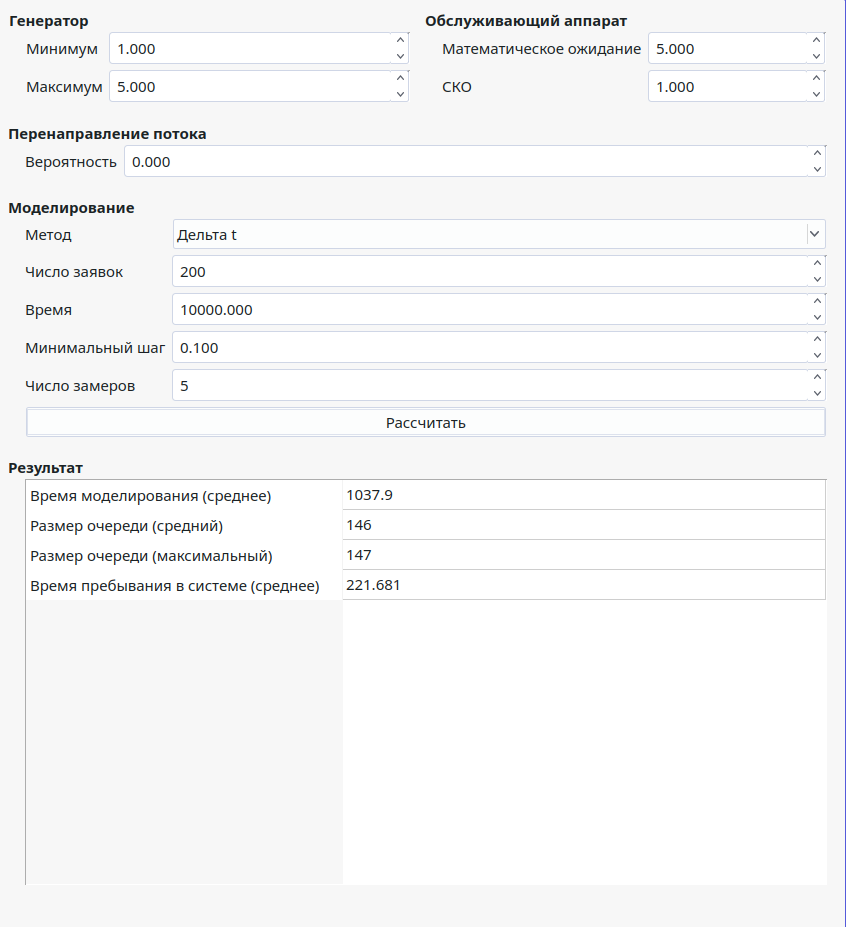
\includegraphics[width=\linewidth]{dtp0n200.png}
    \end{minipage}
    \hfill
    \begin{minipage}{0.45\textwidth}
        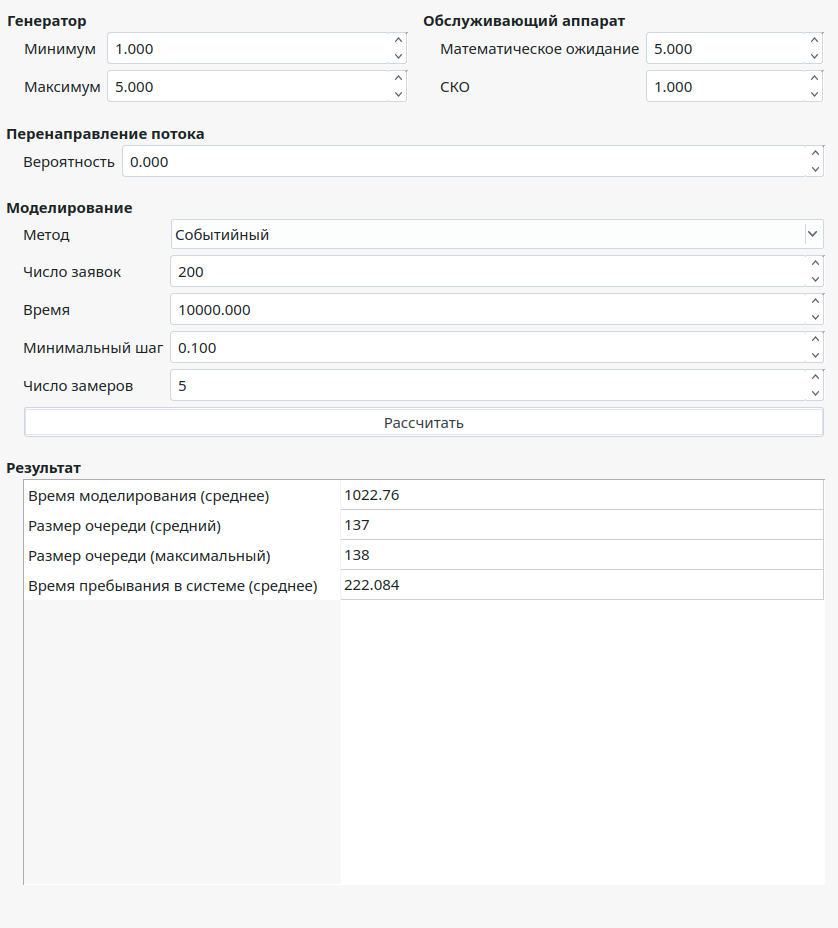
\includegraphics[width=\linewidth]{eventp0n200.png}
    \end{minipage}
    \begin{center}
        Ожидаемое время моделирования: 1000
    \end{center}
    \caption{Результаты работы для $a=1, b=5, \mu=5, \sigma=1, p=0, n=200$}
\end{figure}

\begin{figure}[h]
    \begin{minipage}{0.45\textwidth}
        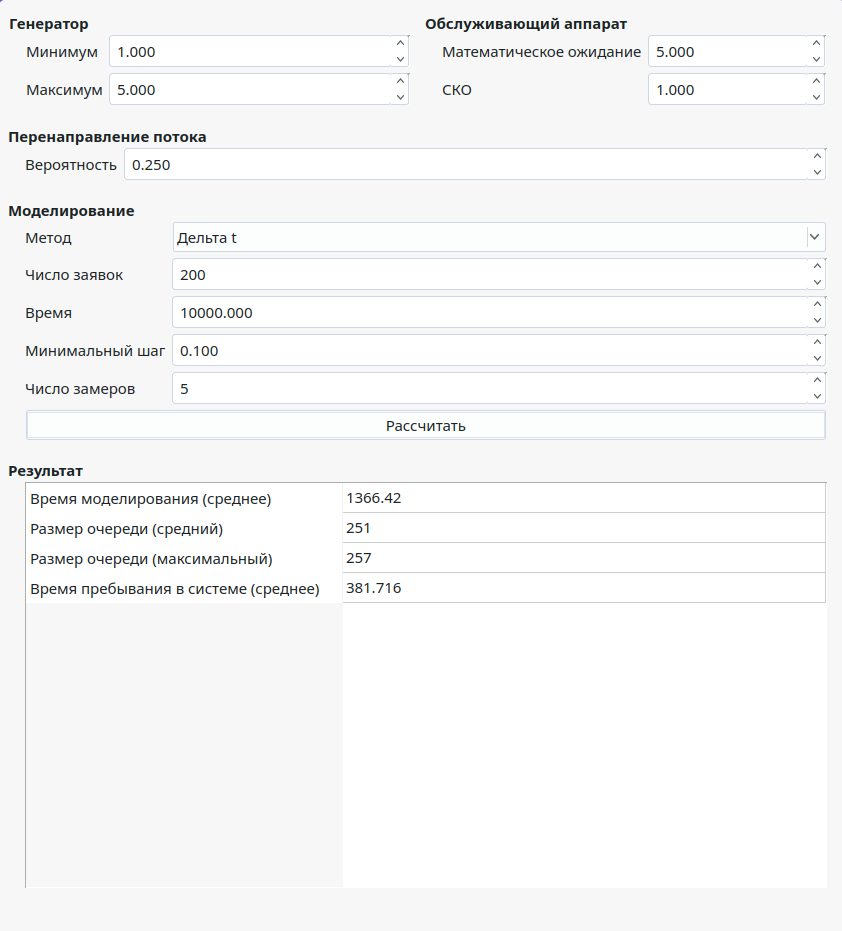
\includegraphics[width=\linewidth]{dtp025n200.png}
    \end{minipage}
    \hfill
    \begin{minipage}{0.45\textwidth}
        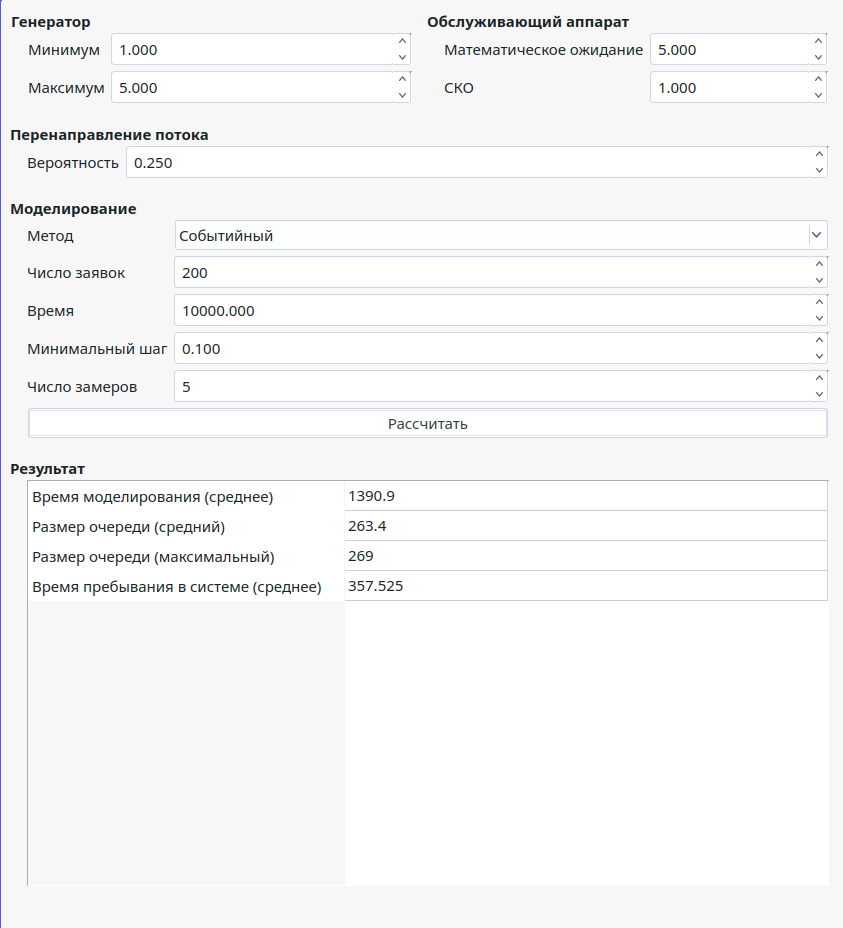
\includegraphics[width=\linewidth]{eventp025n200.png}
    \end{minipage}
    \begin{center}
        Ожидаемое время моделирования: 1333.33
    \end{center}
    \caption{Результаты работы для $a=1, b=5, \mu=5, \sigma=1, p=0.25, n=200$}
\end{figure}

\begin{figure}[h]
    \begin{minipage}{0.45\textwidth}
        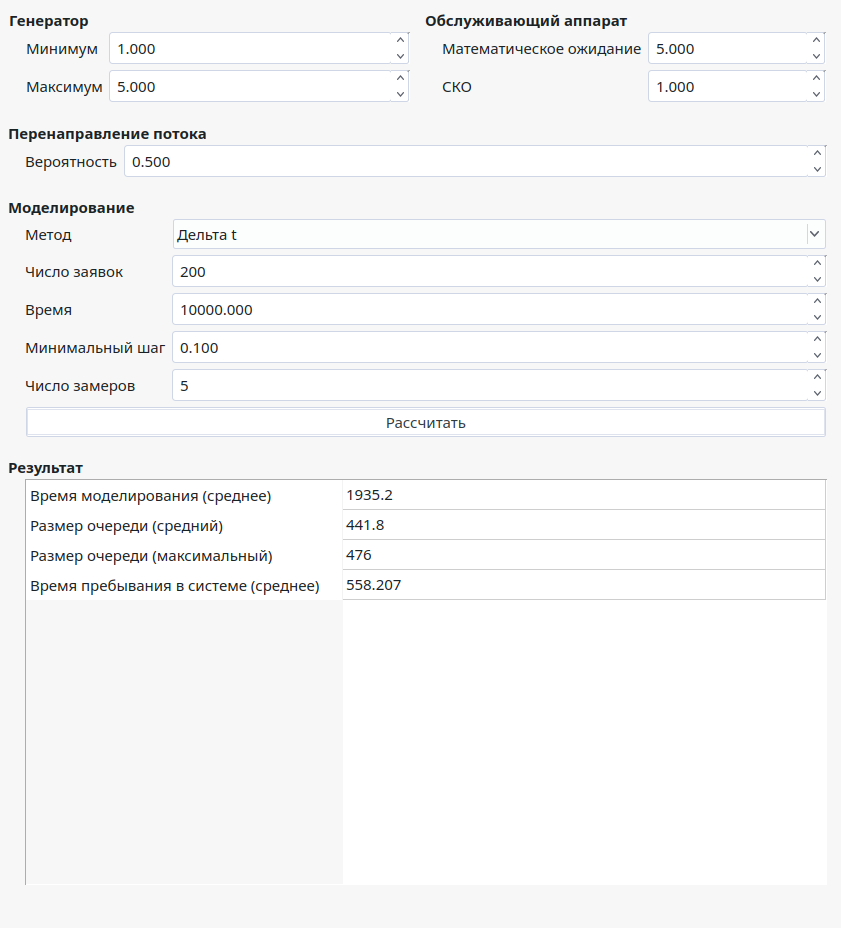
\includegraphics[width=\linewidth]{dtp05n200.png}
    \end{minipage}
    \hfill
    \begin{minipage}{0.45\textwidth}
        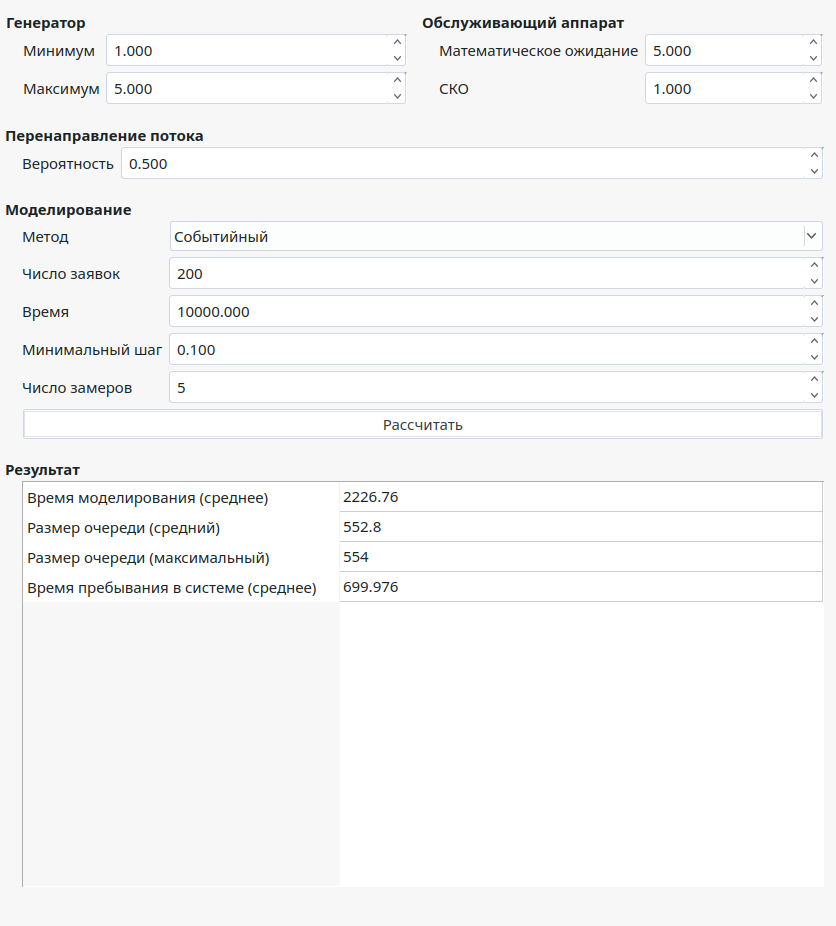
\includegraphics[width=\linewidth]{eventp05n200.png}
    \end{minipage}
    \begin{center}
        Ожидаемое время моделирования: 2000
    \end{center}
    \caption{Результаты работы для $a=1, b=5, \mu=5, \sigma=1, p=0.5, n=200$}
\end{figure}

\begin{figure}[h]
    \begin{minipage}{0.45\textwidth}
        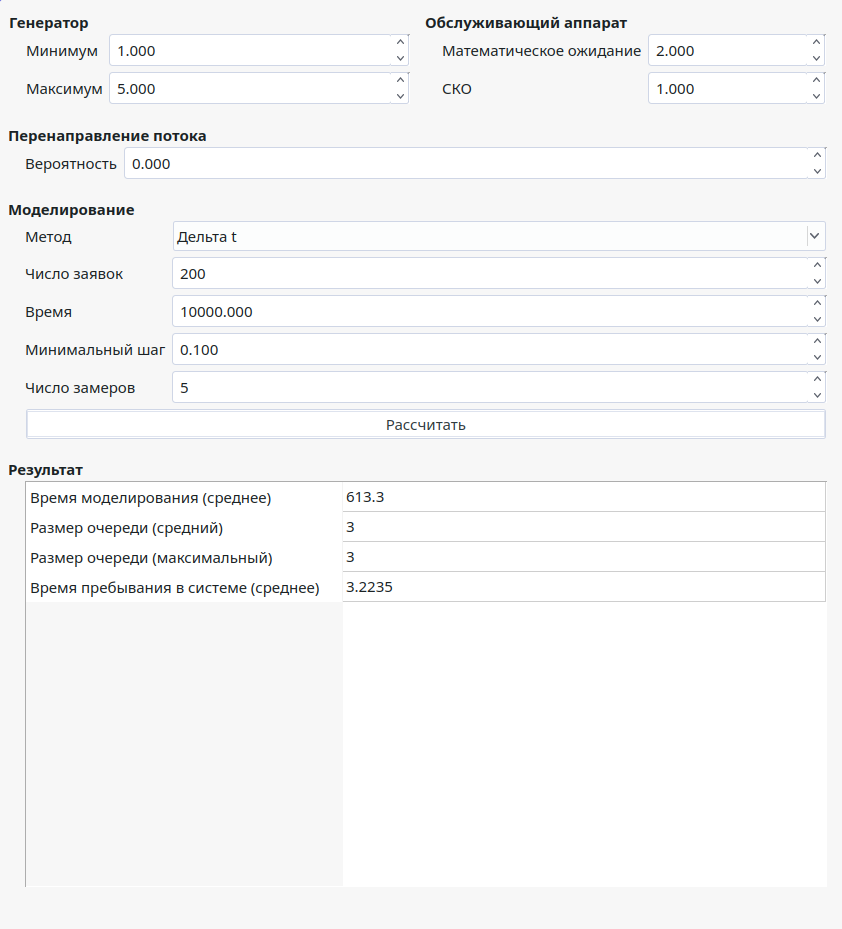
\includegraphics[width=\linewidth]{dt2p0n200.png}
    \end{minipage}
    \hfill
    \begin{minipage}{0.45\textwidth}
        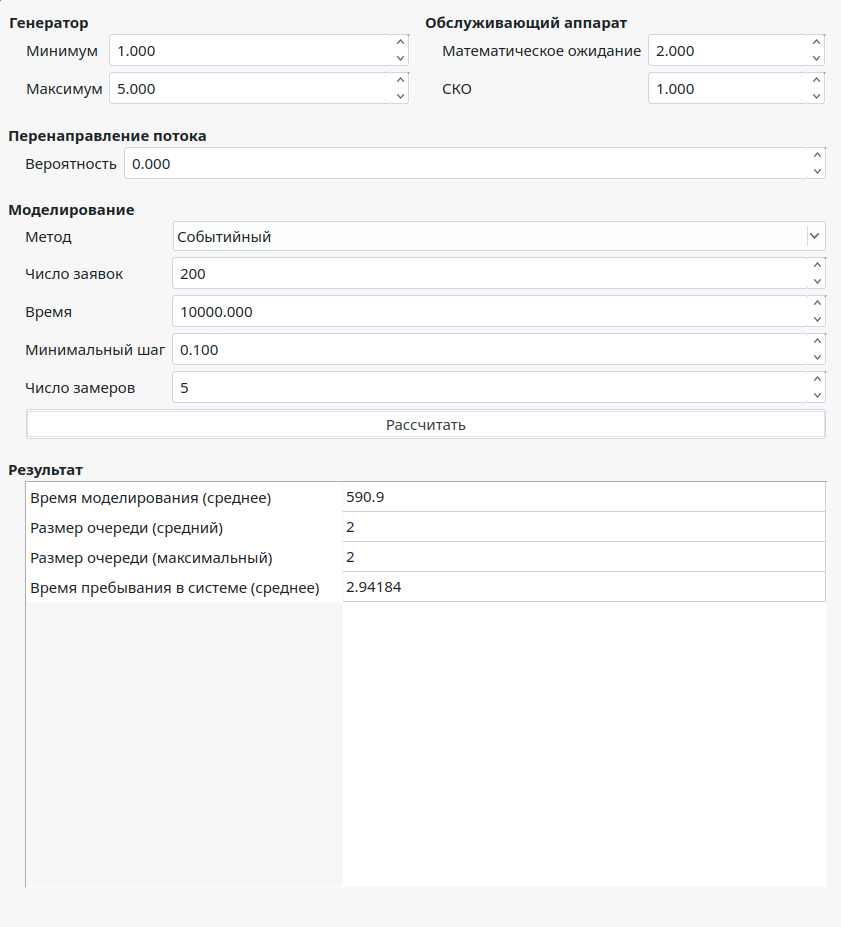
\includegraphics[width=\linewidth]{event2p0n200.png}
    \end{minipage}
    \begin{center}
        Ожидаемое время моделирования: 600
    \end{center}
    \caption{Результаты работы для $a=1, b=5, \mu=2, \sigma=1, p=0, n=200$}
\end{figure}

\begin{figure}[h]
    \begin{minipage}{0.45\textwidth}
        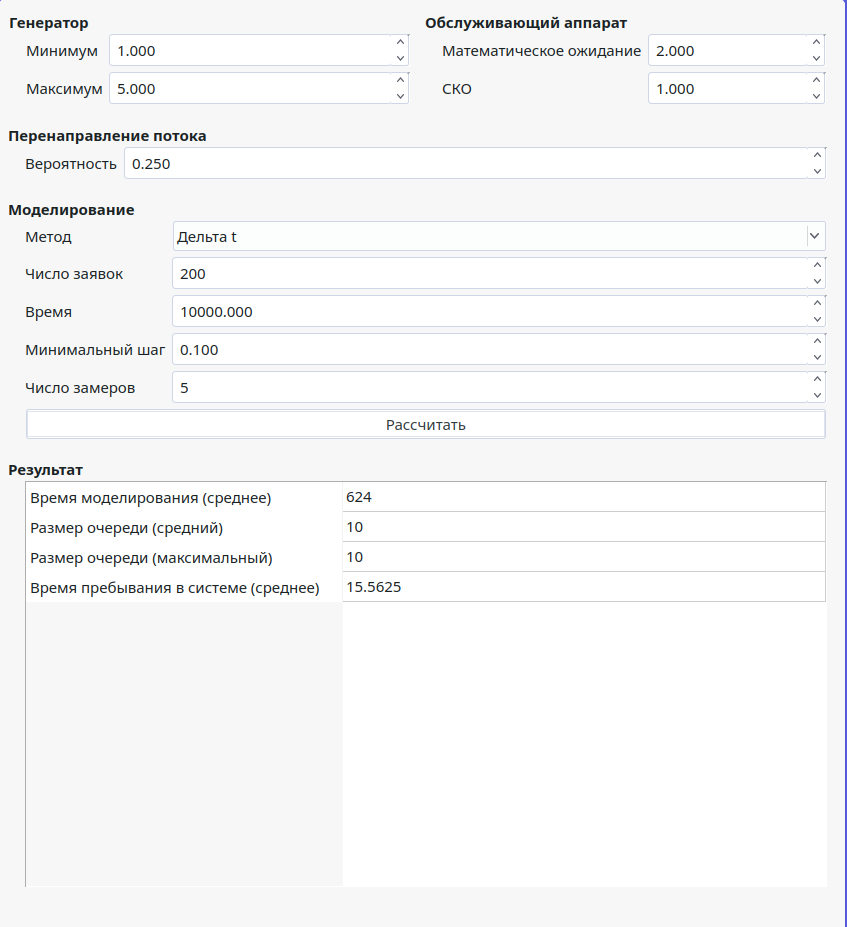
\includegraphics[width=\linewidth]{dt2p025n200.png}
    \end{minipage}
    \hfill
    \begin{minipage}{0.45\textwidth}
        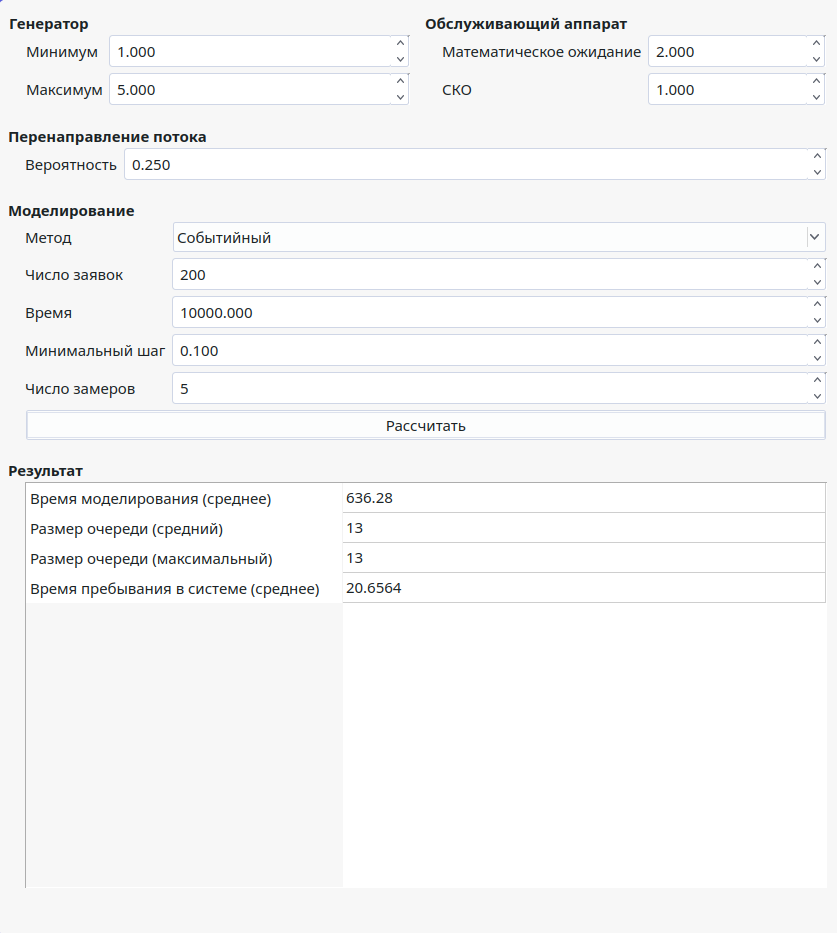
\includegraphics[width=\linewidth]{event2p025n200.png}
    \end{minipage}
    \begin{center}
        Ожидаемое время моделирования: 600
    \end{center}
    \caption{Результаты работы для $a=1, b=5, \mu=2, \sigma=1, p=0.25, n=200$}
\end{figure}

\begin{figure}[h]
    \begin{minipage}{0.45\textwidth}
        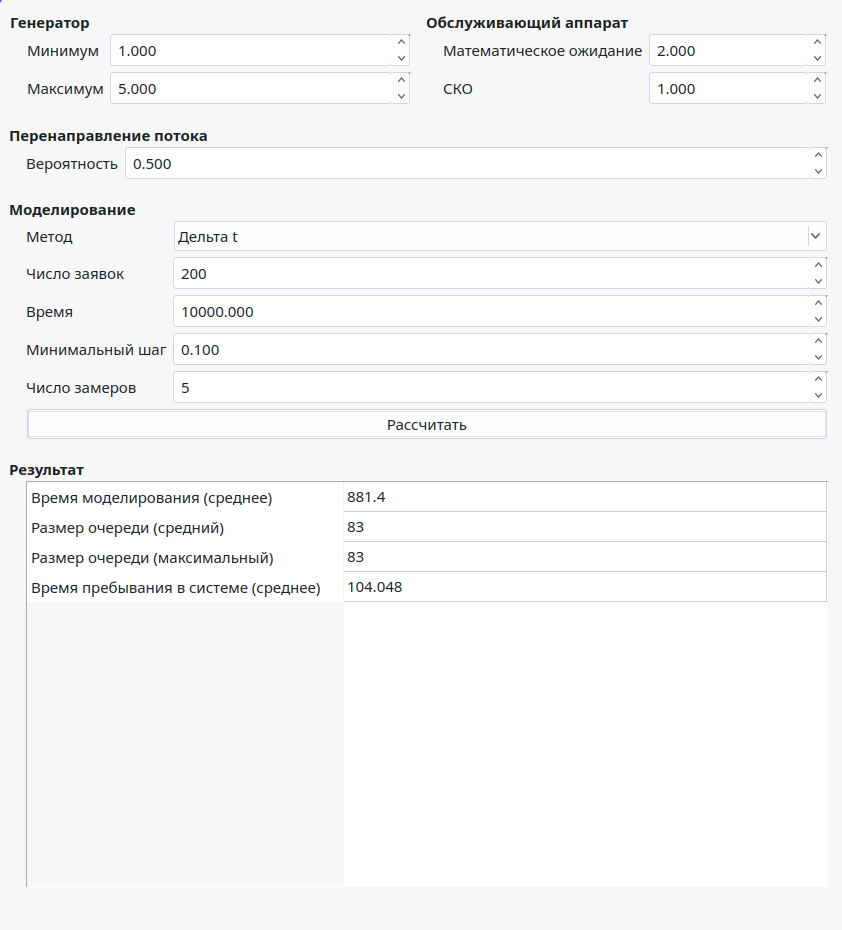
\includegraphics[width=\linewidth]{dt2p05n200.png}
    \end{minipage}
    \hfill
    \begin{minipage}{0.45\textwidth}
        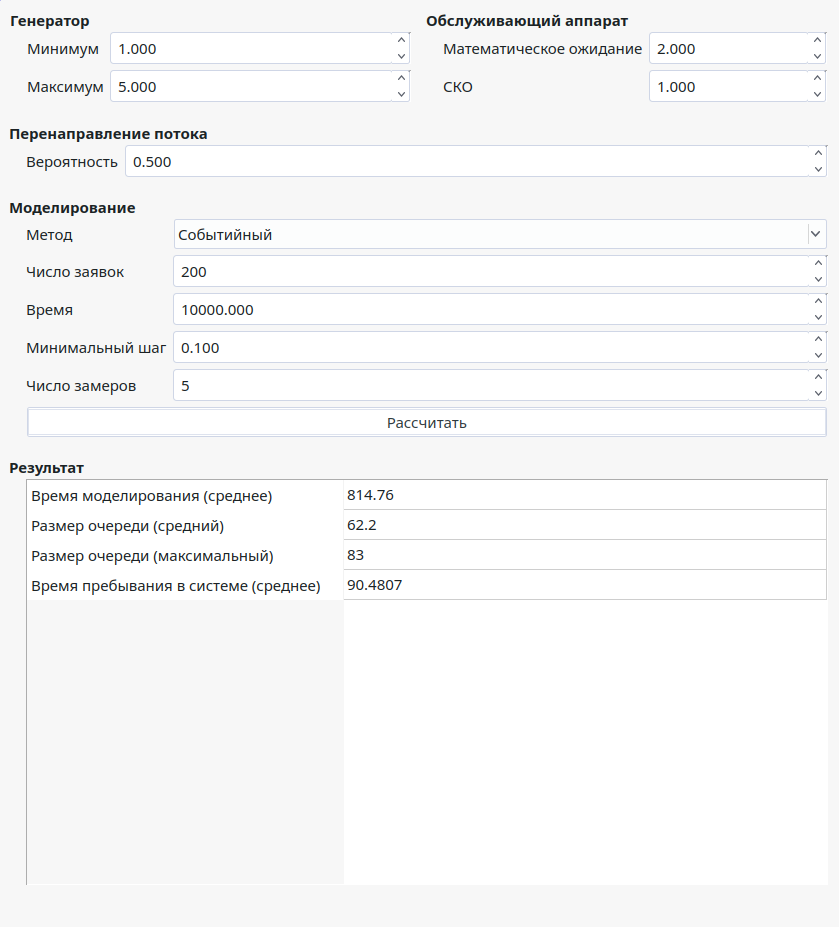
\includegraphics[width=\linewidth]{event2p05n200.png}
    \end{minipage}
    \begin{center}
        Ожидаемое время моделирования: 800
    \end{center}
    \caption{Результаты работы для $a=1, b=5, \mu=2, \sigma=1, p=0.5, n=200$}
\end{figure}

% \begin{figure}[h]
%     \begin{minipage}{0.3\textwidth}
%         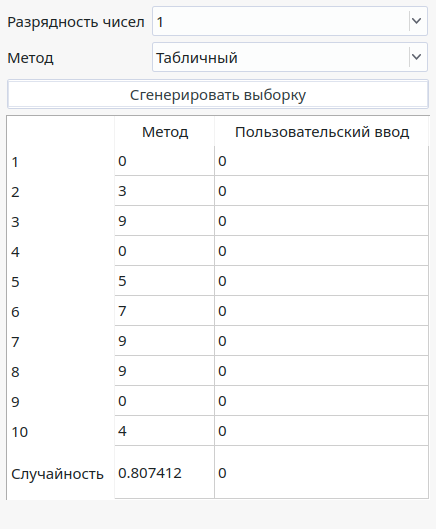
\includegraphics[width=\linewidth]{4.png}
%     \end{minipage}
%     \hfill
%     \begin{minipage}{0.3\textwidth}
%         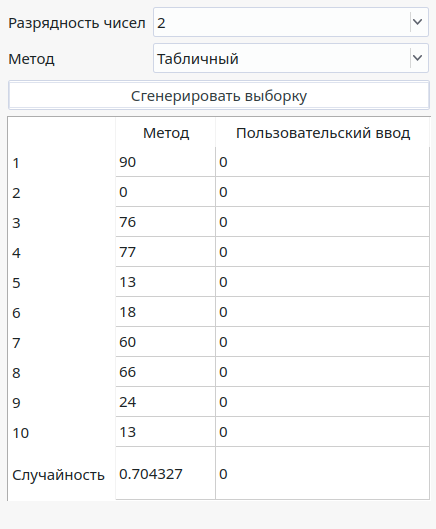
\includegraphics[width=\linewidth]{5.png}
%     \end{minipage}
%     \hfill
%     \begin{minipage}{0.3\textwidth}
%         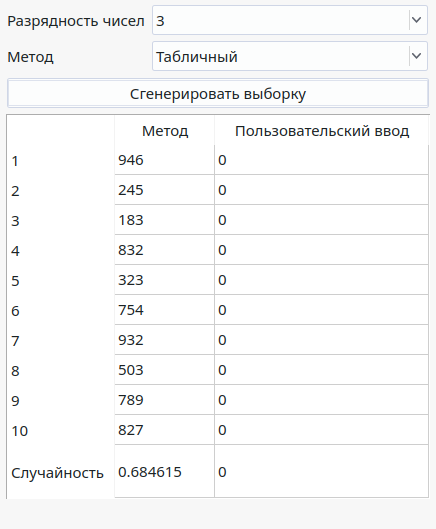
\includegraphics[width=\linewidth]{6.png}
%     \end{minipage}
%     \caption{Результаты работы программы для табличного метода}
% \end{figure}

\clearpage

\section*{Вывод}

В ходе выполнения работы была промоделирована системы, состоящей из генератора,
буфера и обслуживающего аппарата с использованием методов протягивания
модельного времени ($\Delta t$ и событийный). Была рассмотрена зависимость длины
очереди от параметров системы.

